\chapter{Internship tasks }
\section{Problem}
At the moment, the light duty air compressor market mainly use electricity as the power source, which can be inconvenient at remote locations where power grid is difficult to reach. To solve this problem, we will analyze and model a V-twin air compressor with a compression end and a combustion end. The model is programmed using MATLAB\textsuperscript{\textregistered} R2019a.
\section{Parameters}
\begin{figure}
	\centering
	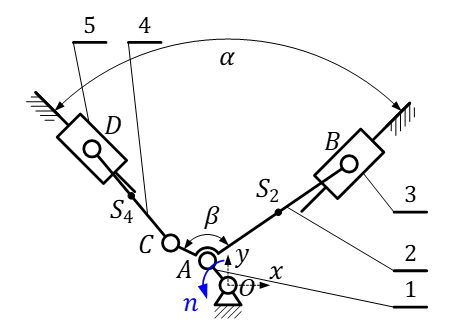
\includegraphics[width=0.5\linewidth]{03}
	\caption{Mechanism of the air compressor}
	\label{fig:03}
\end{figure}
\begin{tabular}{p{9cm}p{6cm}}
	Piston lift & $ H_C=39\unit{mm} $\\
	V-angle&$ \alpha=90^\circ $\\
	Connecting rod dimensions  &$ \dfrac{l_{AB}}{l_{OA}} =5.372,l_{AC}=25mm$, $\beta=120^\circ$\\
	Crankshaft 1 weight&$ m_1=1.6262\unit{kg} $\\
	Center of gravity of link 1&$ S_1\equiv O $\\
	Moment of inertia of link 1&$ J_{s1}=0.0045585\unit{kg\cdot m^2} $\\
	Connecting rod 2 weight&$ m_2=0.29597\unit{kg} $\\
	Center of gravity of link 2&$ l_{AS2}=l_{S2B} $\\
	Moment of inertia of link 2&$ J_{S2}=0.004874\unit{kg\cdot m^2} $\\
	Connecting rod 4 weight&$ m_2=0.13865\unit{kg} $\\
	Center of gravity of link 4&$ l_{CS4}=l_{S4D} $\\
	Moment of inertia of link 4&$ J_{S4}=0.00011121\unit{kg\cdot m^2} $\\
	Piston weight&$ m_3=m_5=0.33513\unit{kg} $\\
	Center of gravity of link 3 and 5&$ S_3\equiv B, S_5\equiv D $\\
	Piston crown area&$ A=0.01\unit{m^2} $\\
	Maximum operating pressure (The graphs given in figure \ref{fig:2a} and \ref{fig:2b})&$ p_{max}=23\unit{bar} $\\
	Allowable tolerance factor&$ \delta=1/80 $\\
	Average rotational velocity&$ n_1=500\unit{rpm} $\\
	Valve lift (trapezoidal acceleration)&$ s_0=2\unit{mm} $ \\
	Early opening and late closing of combustion end&$ 25^\circ $\\
	Early opening of compression end&$ 40^\circ $\\
	Pressure angle of cam follower&$ \alpha_2=6^\circ $\\
	Periodic angles&$ \phi_{rise}=\phi_{fall}$, $\phi_{rise,comb}=5^\circ$, $\phi_{rise,comp}=20^\circ $
\end{tabular}
\begin{figure}
	\centering
	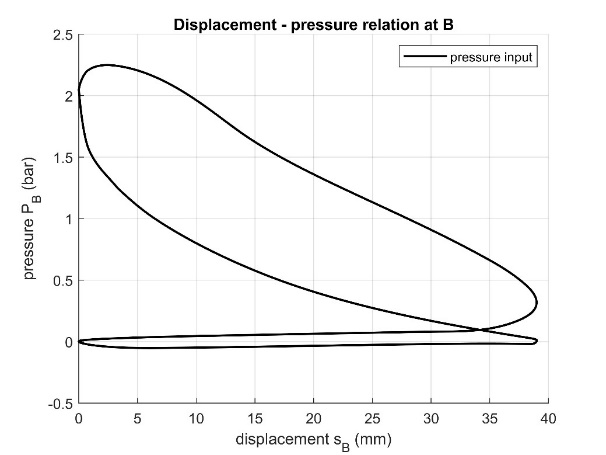
\includegraphics[width=0.7\linewidth]{2.2a}
	\caption{Pressure graph at link 3 (not to scale)}
	\label{fig:2a}
\end{figure}
\begin{figure}
	\centering
	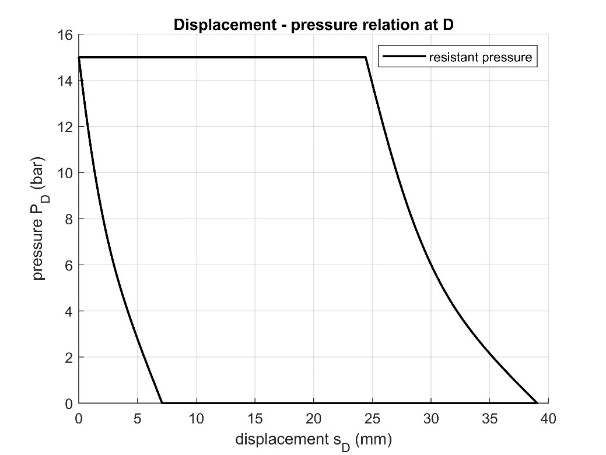
\includegraphics[width=0.7\linewidth]{2.2b}
	\caption{Pressure graph at link 5 (not to scale)}
	\label{fig:2b}
\end{figure}
\section{Objectives}
\begin{enumerate}
	\item Mechanism synthesis \cite{li_1984_hng}
	\item Kinematic analysis of the mechanism
	\item Force  analysis of the mechanism
	\item Identify energy relation and calculate the flywheel weight
	\item Combining the motion
	\item Model cam mechanism for compression piston
\end{enumerate}
\section{Displacement analysis}
\paragraph{Position of $ A $}
\begin{equation}\label{rA}
\vec{r}_A=
\matgen{x_A}{y_A}{0}=\matgen{l_{OA}\cos \phi}{l_{OA}\sin \phi}{0}
\end{equation}
where $ \phi=\widehat {xOA} $
\paragraph{Position of $ B $}
\begin{equation}\label{rB}
	\left\{
		\begin{array}{cl}
		(x_A-x_B)^2+(y_A-y_B)^2&=l_{AB}^2\\
		\dfrac{y_B}{x_B}&=\tan \widehat{xOB}\\
		\end{array}
	\right.
\end{equation}
Solve equation (\ref{rB}) yields 2 positions $ B_1, B_2 $. Combining with condition $ x_B,y_B>0 $ to find the correct solution.
\[\vec{r}_B=
\matgen{x_B}{y_B}{0}\]
\paragraph{Position of $ C $}
\begin{equation}\label{rC}
\left\{
\begin{array}{cl}
(x_A-x_C)^2+(y_A-y_C)^2&=l_{AC}^2\\
(x_B-x_C)^2+(y_B-y_C)^2&=l_{BC}^2\\
\end{array}
\right.
\end{equation}
Solve equation (\ref{rC}) yields 2 sets of positions $ C_1, C_2 $, one of which is the correct solution. This can be programmed using MATLAB\textup{\textregistered} to try both sets.
\[\vec{r}_C=
\matgen{x_C}{y_C}{0}\]
\paragraph{Position of $ D $}
\begin{equation}\label{rD}
\left\{
\begin{array}{cl}
(x_C-x_D)^2+(y_C-y_D)^2&=l_{CD}^2\\
\dfrac{y_D}{x_D}&=\tan \widehat{xOD}\\
\end{array}
\right.
\end{equation}
Solve equation (\ref{rD}) yields 2 positions $ D_1, D_2 $. Combining with condition $ x_D<0,y_D>0 $ to find the correct solution.
\[\vec{r}_D=
\matgen{x_D}{y_D}{0}\]
\begin{figure}
	\centering
	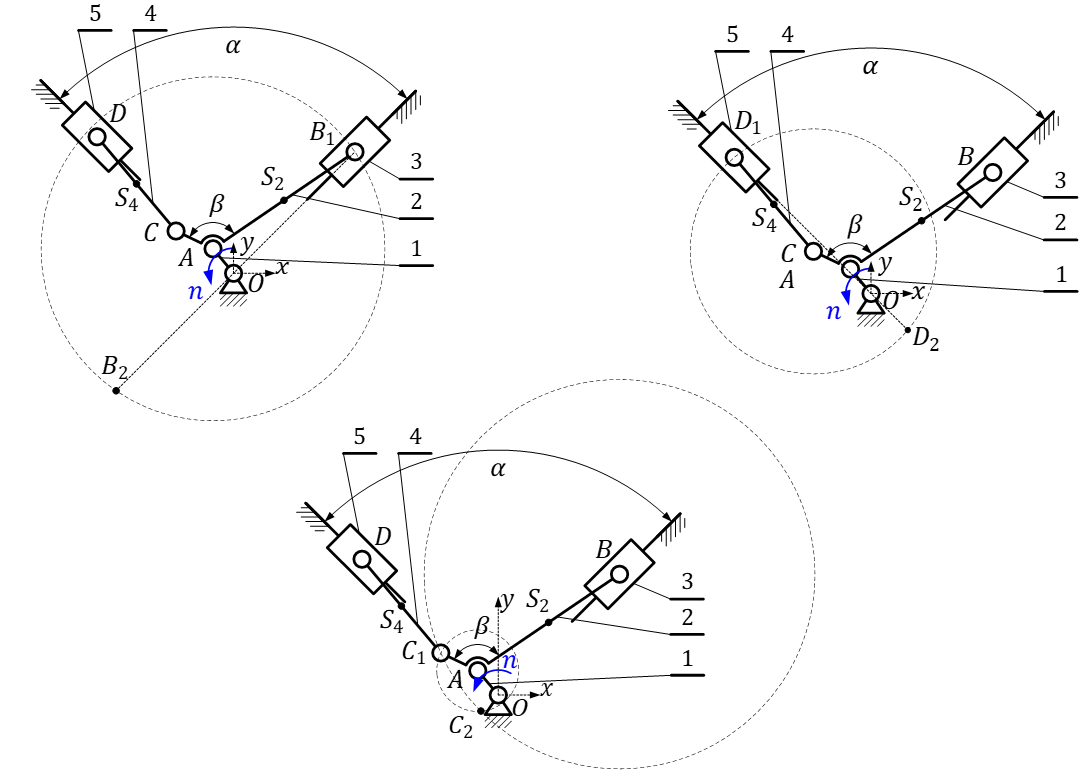
\includegraphics[width=0.8\linewidth]{04}
	\caption{Position analysis of $B$, $C$ and $D$}
	\label{fig:04}
\end{figure}
Using MATLAB\textup{\textregistered} to plot the positions of the mechanism in figure \ref{fig:05}
\begin{figure}
	\centering
	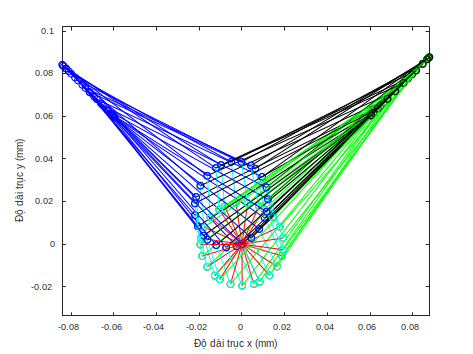
\includegraphics[width=0.7\linewidth]{05}
	\caption{Locus of the mechanism using MATLAB\textup{\textregistered}}
	\label{fig:05}
\end{figure}
\section{Velocity and Acceleration analysis}
With the analytical solutions of the points $ A,B,C,D $, we can easily find the corresponding velocities and accelerations using derivative with respect to time $ t $. Also, we need to remember that $ \phi(t) $ is a time-dependent variable.
\subsection{Velocity analysis}
\paragraph{Velocity of $ A $}
\begin{equation}\label{vA}
\vec{v}_A=\dot{\vec{r}}_A=\dfrac{d\vec{r}_A}{dt}
\end{equation}
where $ \phi=\widehat{xOA} $
\paragraph{Velocity of $ B $}
\begin{equation}\label{vB}
\vec{v}_B=\dot{\vec{r}}_B=\dfrac{d\vec{r}_B}{dt}=\vec{v}_A+\vec{\omega}_2\times(\vec{r}_B-\vec{r}_A)
\end{equation}
From equation (\ref{vB}), we solve analytically for $ \vec{\omega}_2 $
\[\vec{\omega}_2=\matgen{0}{0}{\omega_2}\]
\paragraph{Velocity of $ C $}
\begin{equation}\label{vC}
\vec{v}_C=\dot{\vec{r}}_C=\dfrac{d\vec{r}_C}{dt}
\end{equation}
\paragraph{Velocity of $ D $}
\begin{equation}\label{vD}
\vec{v}_D=\dot{\vec{r}}_D=\dfrac{d\vec{r}_D}{dt}=\vec{v}_C+\vec{\omega}_4\times(\vec{r}_D-\vec{r}_C)
\end{equation}
From equation (\ref{vD}), we solve analytically for $ \vec{\omega}_4 $
\[\vec{\omega}_4=\matgen{0}{0}{\omega_4}\]
Using MATLAB\textup{\textregistered} to plot the velocity graph of the mechanism in figure \ref{fig:06} \cite{marghitu_2009_mechanisms}. \clearpage
\begin{figure}[h]
	\centering
	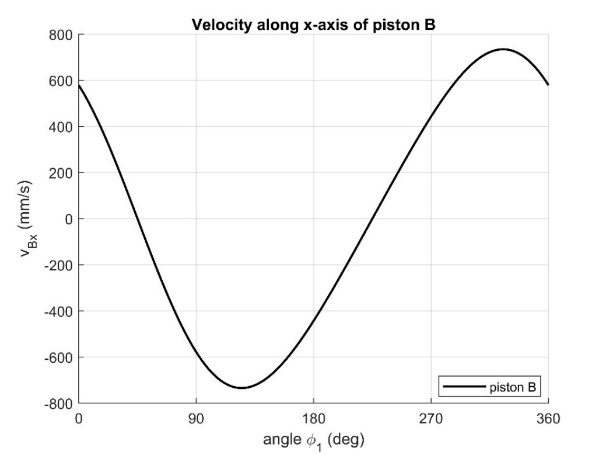
\includegraphics[width=0.7\linewidth]{06}
	\caption{Velocity of link 3}
	\label{fig:06}
\end{figure}
\subsection{Acceleration analysis}
\paragraph{Acceleration of $ A $}
\begin{equation}\label{aA}
\vec{a}_A=\dot{\vec{v}}_A=\dfrac{d\vec{v}_A}{dt}
\end{equation}
where $ \phi=\widehat{xOA} $
\paragraph{Acceleration of $ B $}
\begin{equation}\label{aB}
\vec{a}_B=\dot{\vec{v}}_B=\dfrac{d\vec{v}_B}{dt}
\end{equation}
\[\vec{\alpha}_2=\dfrac{d\vec{\omega}_2}{dt}\]
\paragraph{Acceleration of $ C $}
\begin{equation}\label{aC}
\vec{a}_C=\dot{\vec{v}}_C=\dfrac{d\vec{v}_C}{dt}
\end{equation}
\paragraph{Acceleration of $ D $}
\begin{equation}\label{aD}
\vec{a}_D=\dot{\vec{v}}_D=\dfrac{d\vec{v}_D}{dt}
\end{equation}
\[\vec{\alpha}_4=\dfrac{d\vec{\omega}_4}{dt}\]
Using MATLAB\textup{\textregistered} to plot the acceleration graph of the mechanism in figures \ref{fig:07}
\begin{figure}[h]
	\centering
	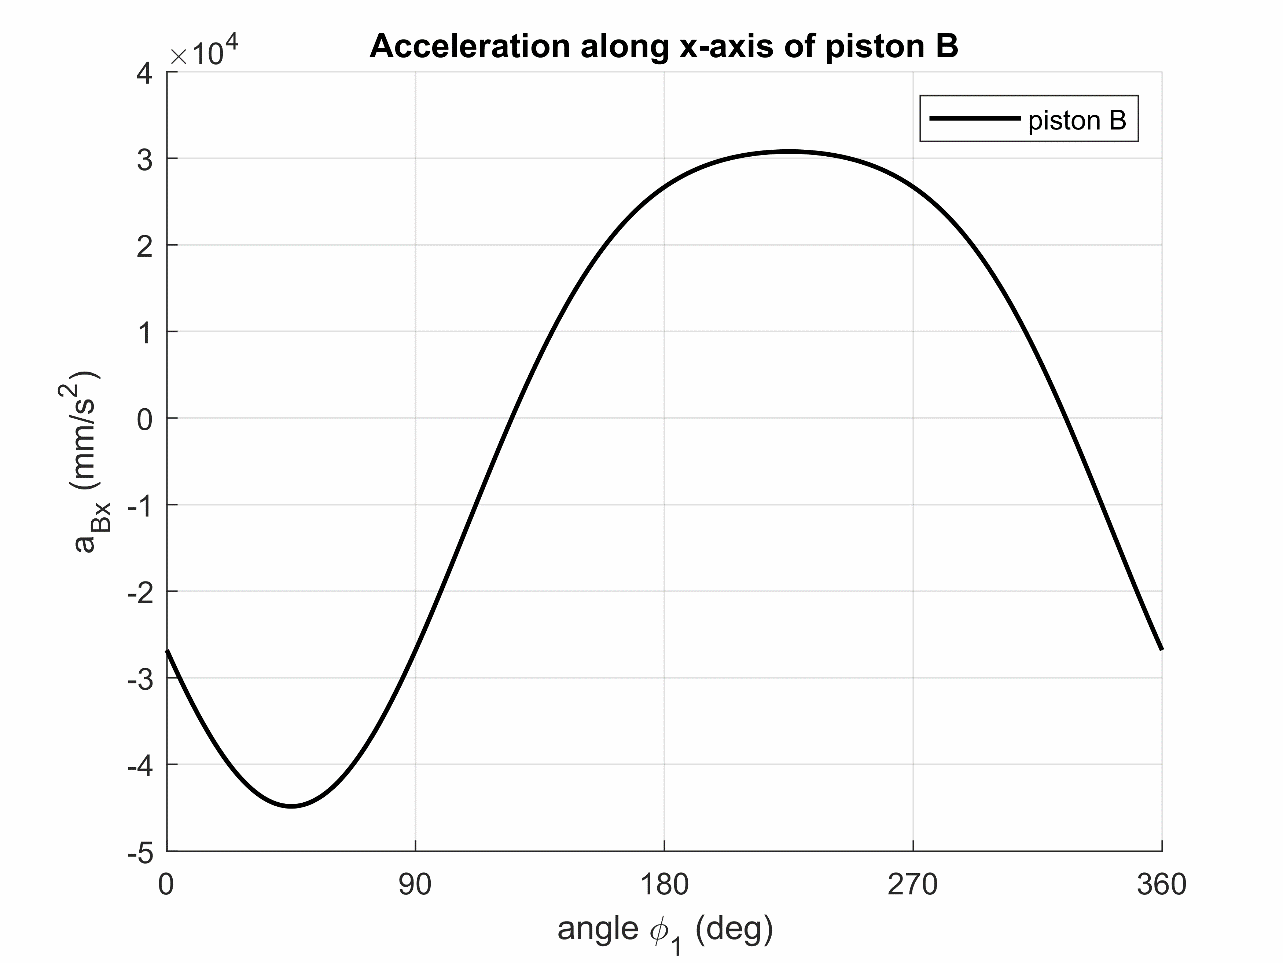
\includegraphics[width=0.7\linewidth]{07}
	\caption{Acceleration of link 3}
	\label{fig:07}
\end{figure}
\section{Force analysis}
To find the reaction forces, we separate the links and solve the D'Alembert equations analytically.
\begin{figure}[h]
	\centering
	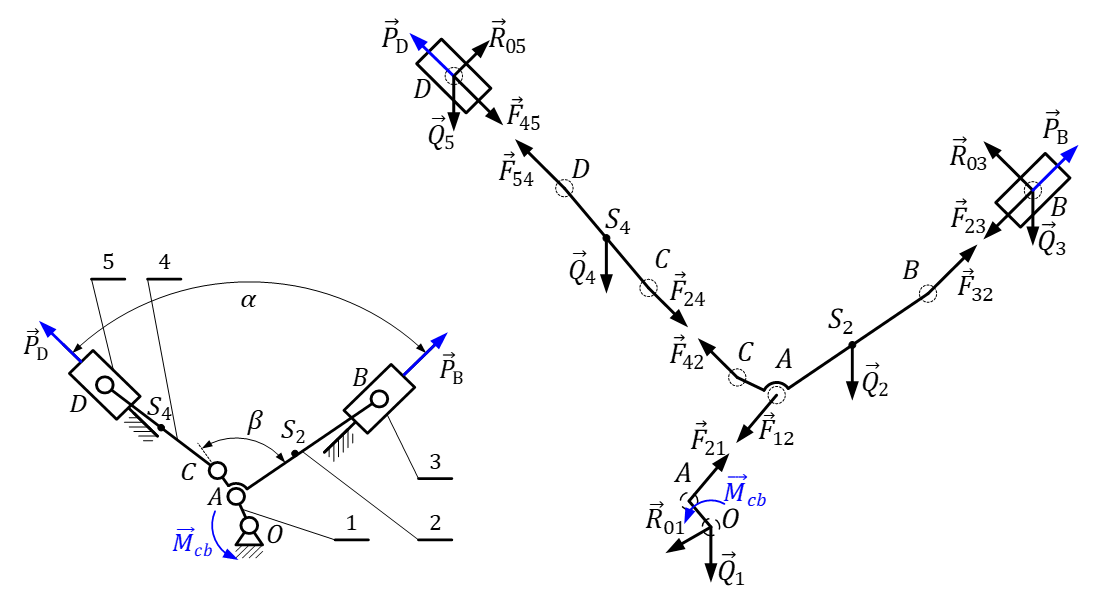
\includegraphics[width=0.8\linewidth]{08}
	\caption{Force analysis of the mechanism}
	\label{fig:08}
\end{figure}\\
Position and acceleration equations of the links, located at their centers of gravity:
\begin{equation}\label{rS}
	\vec{r}_{S1}=\vec{0},\vec{r}_{S2}=\dfrac{\vec{r}_A+\vec{r}_B}{2},\vec{r}_{S4}=\dfrac{\vec{r}_D+\vec{r}_C}{2}
\end{equation}
\begin{equation}
\vec{a}_{S1}=\vec{0},\vec{a}_{S2}=\dfrac{\vec{a}_A+\vec{a}_B}{2},\vec{a}_{S4}=\dfrac{\vec{a}_D+\vec{a}_C}{2}
\end{equation}
The equations for 5 links are systemized as follows:
\paragraph{Link 5}
\begin{equation}
	\left\{
	\begin{array}{cl}
	\vec{Q}_{5}+\vec{F}_{45}+\vec{P}_D+\vec{R}_{05}&=m_5\vec{a}_5\qquad(\vec{a}_5=\vec{a}_D)\\
	\left|\vec{R}_{05x}\right|&=\left|\vec{R}_{05y}\right|
	\end{array} 
	\right.
\end{equation}
\paragraph{Link 4}
\begin{equation}
\left\{
\begin{array}{cl}
\vec{Q}_{4}+\vec{F}_{24}+\vec{F}_{54}&=m_4\vec{a}_{S4}\qquad(\vec{F}_{54}=-\vec{F}_{45})\\
(\vec{r}_D-\vec{r}_{S4})\times \vec{F}_{54}+(\vec{r}_C-\vec{r}_{S4})\times \vec{F}_{24}&=J_{S4}\vec{\alpha}_4
\end{array} 
\right.
\end{equation}
\paragraph{Link 3}
\begin{equation}
\left\{
\begin{array}{cl}
\vec{Q}_{3}+\vec{F}_{23}+\vec{P}_B+\vec{R}_{03}&=m_3\vec{a}_3\\
\left|\vec{R}_{03x}\right|&=-\left|\vec{R}_{03y}\right|
\end{array} 
\right.
\end{equation}
\paragraph{Link 2}
\begin{equation}
	\left\{
	\begin{array}{cl}
	\vec{Q}_{2}+\vec{F}_{12}+\vec{F}_{42}&=m_2\vec{a}_{S2}\\
	(\vec{r}_C-\vec{r}_{S2})\times \vec{F}_{42}+(\vec{r}_B-\vec{r}_{S2})\times \vec{F}_{32}+(\vec{r}_A-\vec{r}_{S2})\times \vec{F}_{12}&=J_{S2}\vec{\alpha}_2
	\end{array} 
	\right.
\end{equation}
where $ \vec{F}_{42}=-\vec{F}_{24}, \vec{F}_{32}=-\vec{F}_{23} $
\paragraph{Link 1}
\begin{equation}\label{L1}
\left\{
\begin{array}{cl}
\vec{Q}_{1}+\vec{F}_{21}+\vec{R}_{01}&=m_1\vec{a}_{S1}\\
\vec{r}_A\times \vec{F}_{21}+\vec{M}_{cb}&=0
\end{array} 
\right.
\end{equation}
Solving for system of equations from (\ref{rS}) to (\ref{L1}) by rearranging them into matrix form, we obtain $ \vec{F}_{45},\vec{R}_{05},\vec{F}_{24},\vec{F}_{23},\vec{F}_{12},\vec{R}_{01},\vec{R}_{03},\vec{M}_{cb} $.\\
Using MATLAB\textup{\textregistered} to plot the reaction force $ \vec{F}_{23},\vec{R}_{03} $ of the mechanism in figures \ref{fig:09} and \ref{fig:10}
\begin{figure}
	\centering
	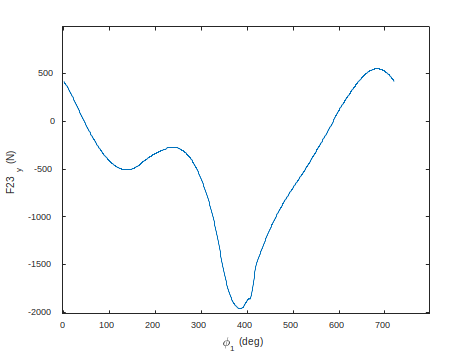
\includegraphics[width=0.7\linewidth]{09}
	\caption{Reaction force $\vec{F}_{23}$ along y axis}
	\label{fig:09}
\end{figure}
\begin{figure}
	\centering
	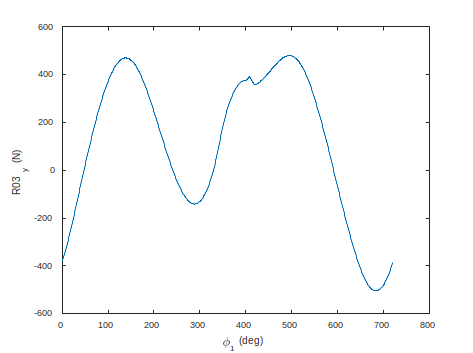
\includegraphics[width=0.7\linewidth]{10}
	\caption{Reaction force $\vec{R}_{03}$ along y axis}
	\label{fig:10}
\end{figure}

\clearpage
\section{Energy relation analysis}
\begin{figure}[h]
	\centering
	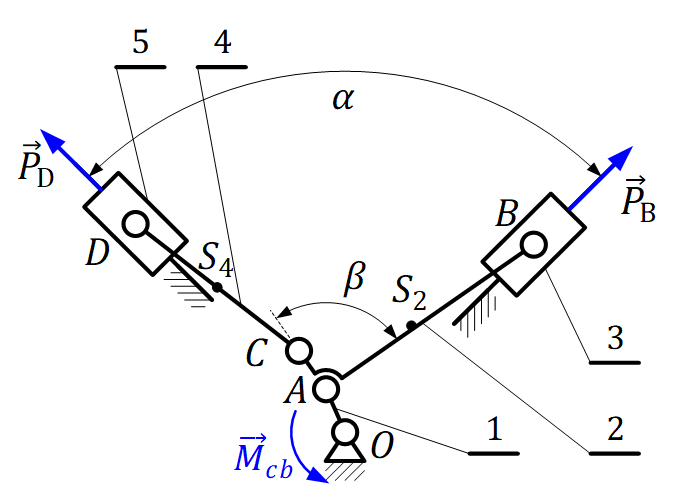
\includegraphics[width=0.4\linewidth]{12}
	\caption{Pressure on both ends of the system}
	\label{fig:12}
\end{figure}
The energy relation of the machine must satisfy the condition such that the motion of the system is regulated after each cycle. To put it another way, the dynamic work is offset by the resistance work: 
\begin{equation}\label{condition}
	\begin{array}{c}
	M_{c}(0)=M_{d}(0)\\
	M_{c}(2\pi)=M_{d}(2\pi)
	\end{array}
\end{equation}
Let us choose the driving link as the equivalent link of the system: $ \omega_{tt}=\omega_1 $.
\subsection{Find equivalent dynamic moment and dynamic work}
From the displacement - pressure relation graph (figure \ref{fig:2a}), we convert it to the external force acting on the system $ F_B(\phi)=P_B(\phi) A $ in a cycle (each displacement data corresponds to a specific position and angle $ \phi(t) $ of the system).
\begin{figure}[h]
	\centering
	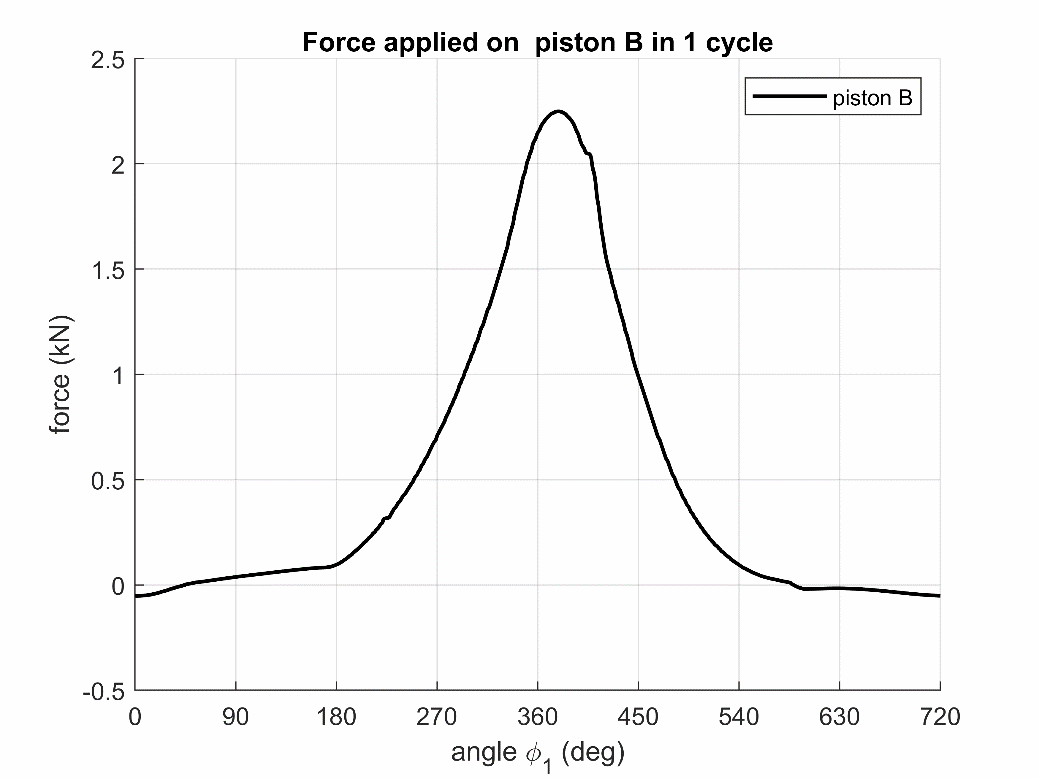
\includegraphics[width=0.6\linewidth]{11}
	\caption{Force applied on piston 3 corresponding to angle of crankshaft 1}
	\label{fig:11}
\end{figure}\\
The equivalent dynamic moment on link 1 is calculated as:
\begin{equation}
	M_d(\phi)=\dfrac{1}{\omega_1}\left(\vec{F}_B\cdot\vec{v}_B+\vec{Q}_2\cdot\vec{v}_{S2}+\vec{Q}_4\cdot\vec{v}_{S4}+\vec{Q}_3\cdot\vec{v}_{B}+\vec{Q}_5\cdot\vec{v}_{D}\right)
\end{equation}
\begin{figure}[h]
	\centering
	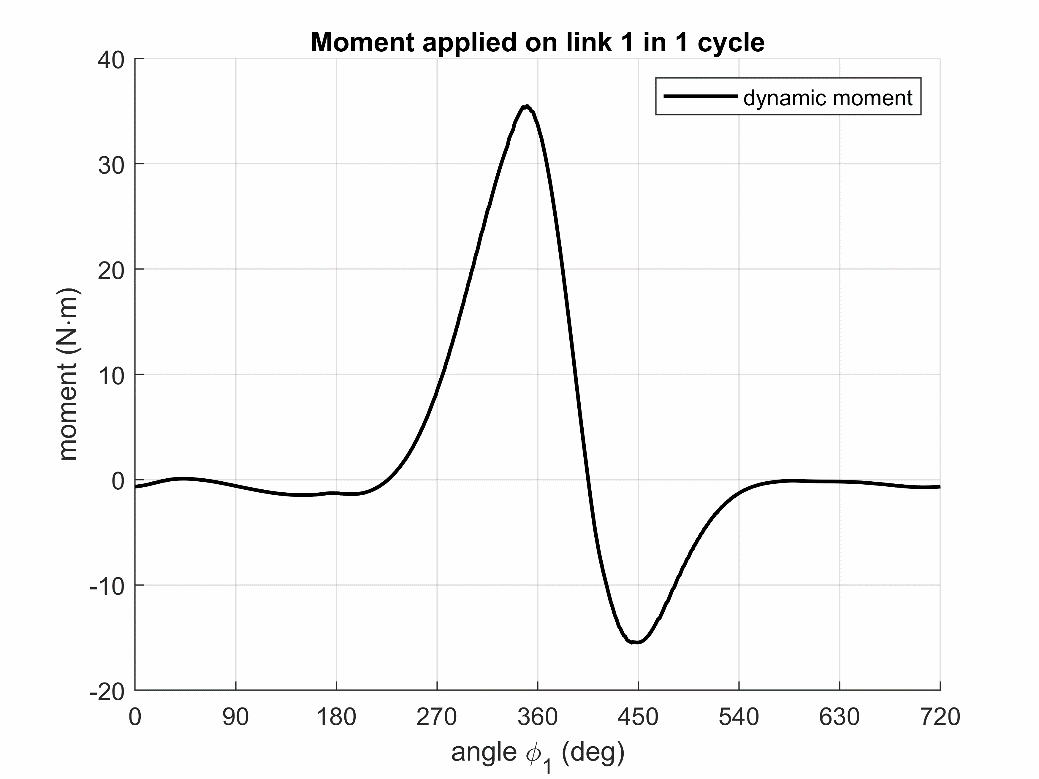
\includegraphics[width=0.6\linewidth]{13}
	\caption{Equivalent dynamic moment applied on crankshaft 1}
	\label{fig:13}
\end{figure}\\
From the moment, we integrate to obtain the dynamic work:
\begin{equation}
	A_d(\phi)=\int_{\phi_i}^{\phi_f}M_d d\phi
\end{equation}
\begin{figure}[h]
	\centering
	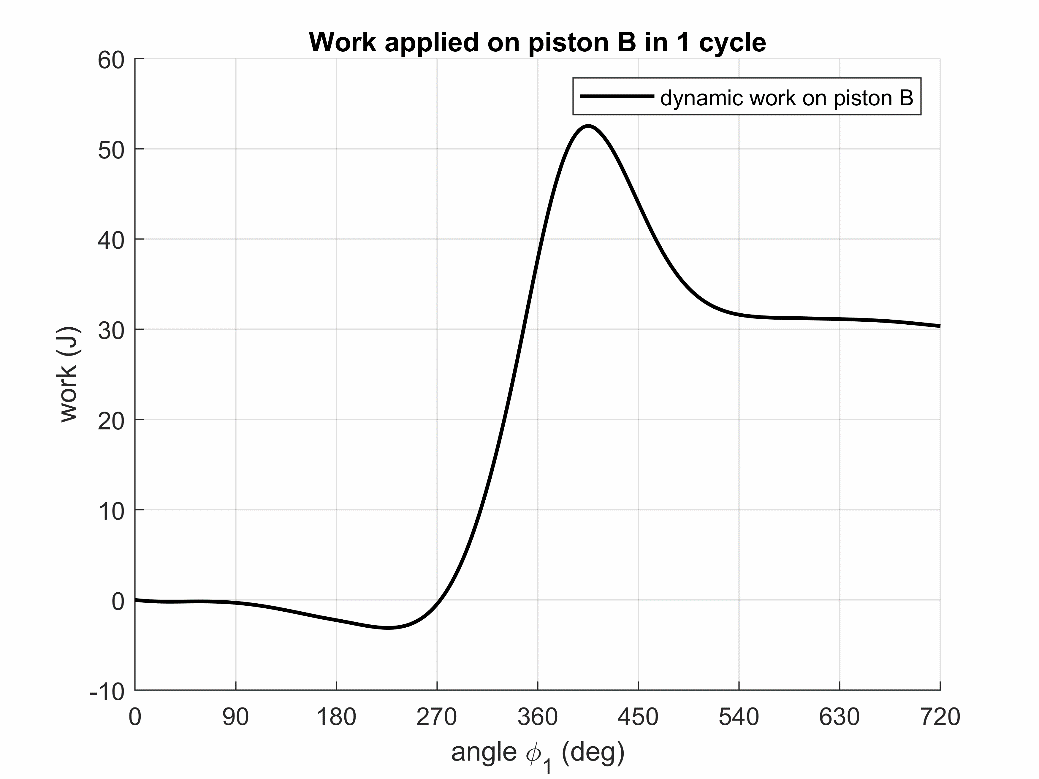
\includegraphics[width=0.6\linewidth]{14}
	\caption{Dynamic work of the system in 1 cycle}
	\label{fig:14}
\end{figure}
\subsection{Find equivalent resistant moment and resistant work}
From the displacement - pressure  relation graph (figure \ref{fig:2b}), we convert it to the external force acting on the system $ F_D(\phi)=P_D(\phi) A $ in a cycle (each displacement data corresponds to a specific position and angle $ \phi(t) $ of the system).
\begin{figure}[h]
	\centering
	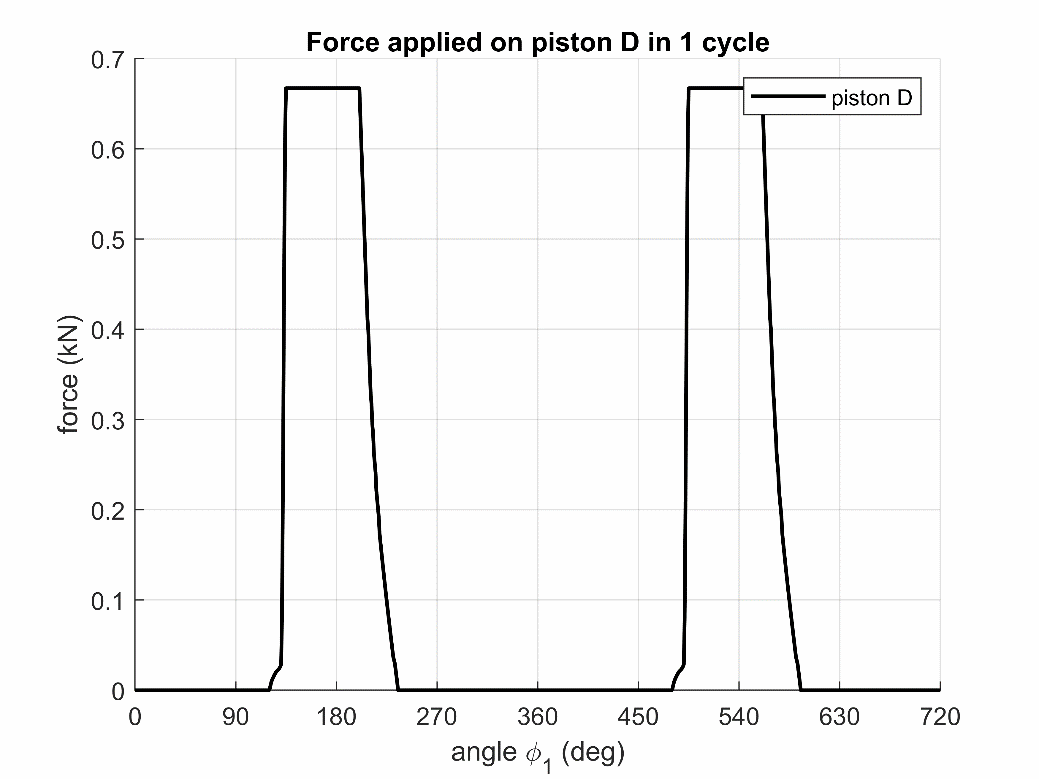
\includegraphics[width=0.6\linewidth]{15}
	\caption{Force applied on piston 3 corresponding to angle of crankshaft 1}
	\label{fig:15}
\end{figure}\\
The equivalent resistant moment on link 1 is calculated as:
\begin{equation}\label{23}
M_c(\phi)=\dfrac{1}{\omega_1}\vec{F}_D\cdot\vec{v}_D
\end{equation}
From the moment, we integrate to obtain the resistant work:
\begin{equation}\label{24}
A_c(\phi)=\int_{\phi_i}^{\phi_f}M_c d\phi
\end{equation}
However, the value of $ M_c $ in equation \ref{23} still does not satisfy condition (\ref{condition}). To compensate for this, we multiply the force $ F_D $ by a ratio $ \dfrac{A_d}{A_c} $ and recalculate $ M_c, A_c $:
\begin{equation}
\begin{array}{l}
F_{D,new}(\phi)=\dfrac{A_d}{A_c}F_D\\
M_{c,new}(\phi)=\dfrac{1}{\omega_1}\vec{F}_{D,new}\cdot\vec{v}_D\\
\displaystyle A_{c,new}(\phi)=\int_{\phi_i}^{\phi_f}M_{c,new} d\phi
\end{array}
\end{equation}\clearpage
We then obtain the figure of equivalent resistant moment and work:
\begin{figure}[h]
	\centering
	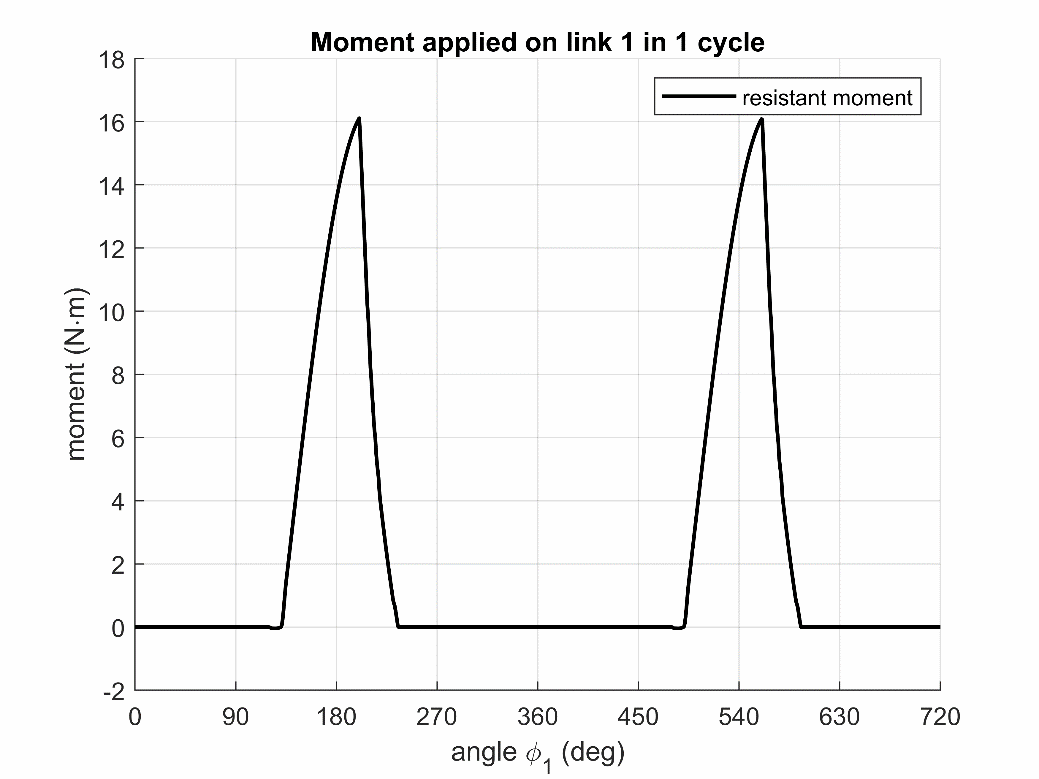
\includegraphics[width=0.66\linewidth]{16}
	\caption{Equivalent resistant moment applied on crankshaft 1}
	\label{fig:16}
\end{figure}
\begin{figure}[h]
	\centering
	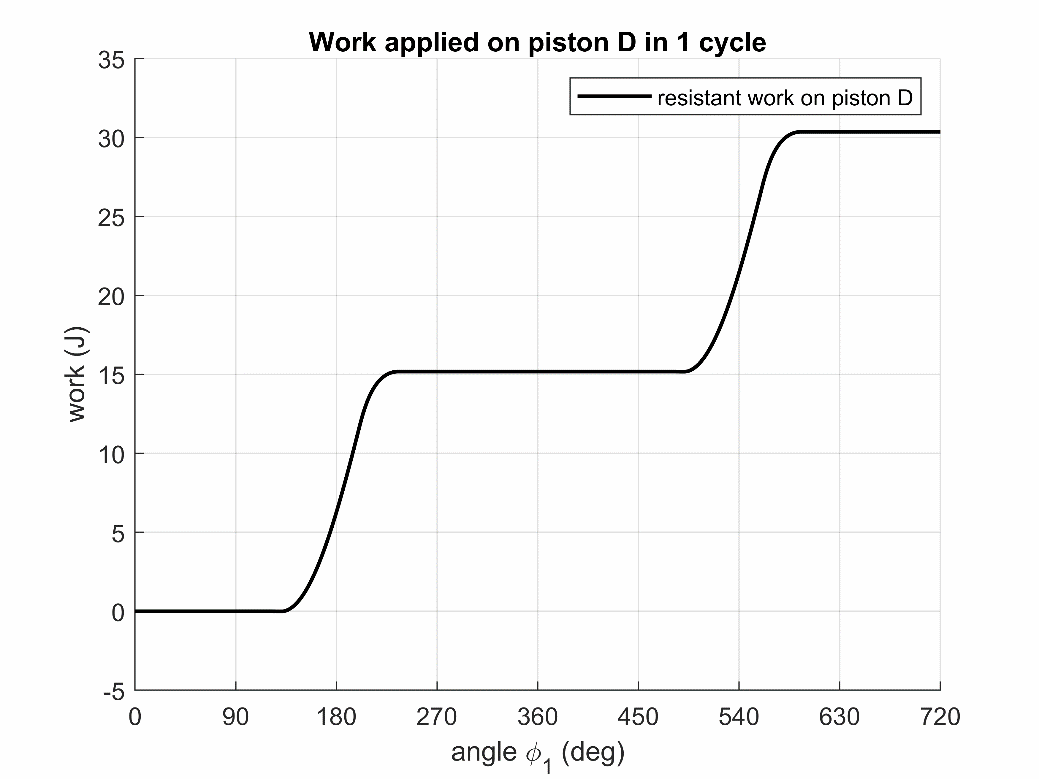
\includegraphics[width=0.66\linewidth]{17}
	\caption{Resistant work of the system in 1 cycle}
	\label{fig:17}
\end{figure}\\
Combining the 2 figures \ref{fig:14} and \ref{fig:17}, we obtain the works applied onto the system in 1 cycle:
\begin{figure}
	\centering
	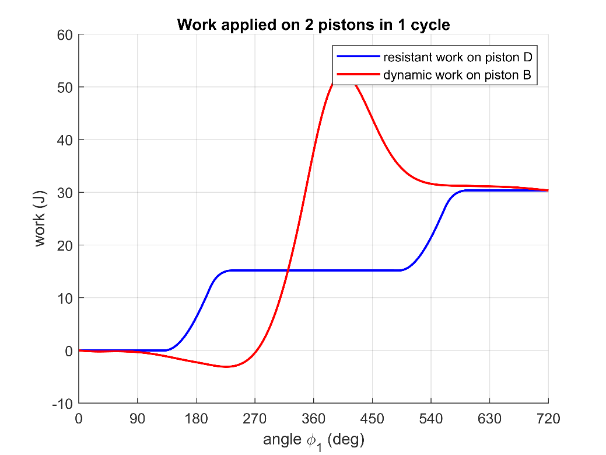
\includegraphics[width=0.6\linewidth]{18}
	\caption{Resistant and dynamic moment of the system in 1 cycle}
	\label{fig:18}
\end{figure}
\section{Find the energy equation and calculate the flywheel weight}
Since the crankshaft is chosen to be the equivalent link, we obtain the equivalent moment of inertia as follows:
\begin{equation}
	J(\phi)=J_1+J_2\left(\dfrac{\omega_2}{\omega_1}\right)^2+m_2\left(\dfrac{v_{S2}}{\omega_1}\right)^2+m_3\left(\dfrac{v_{B}}{\omega_1}\right)^2+J_4\left(\dfrac{\omega_4}{\omega_1}\right)^2+m_5\left(\dfrac{v_{D}}{\omega_1}\right)^2
\end{equation}
where $ m_k,\omega_k,v_k $ are the weight, rotational speed and instantaneous speed at point $ k $ respectively.
\begin{figure}[h]
	\centering
	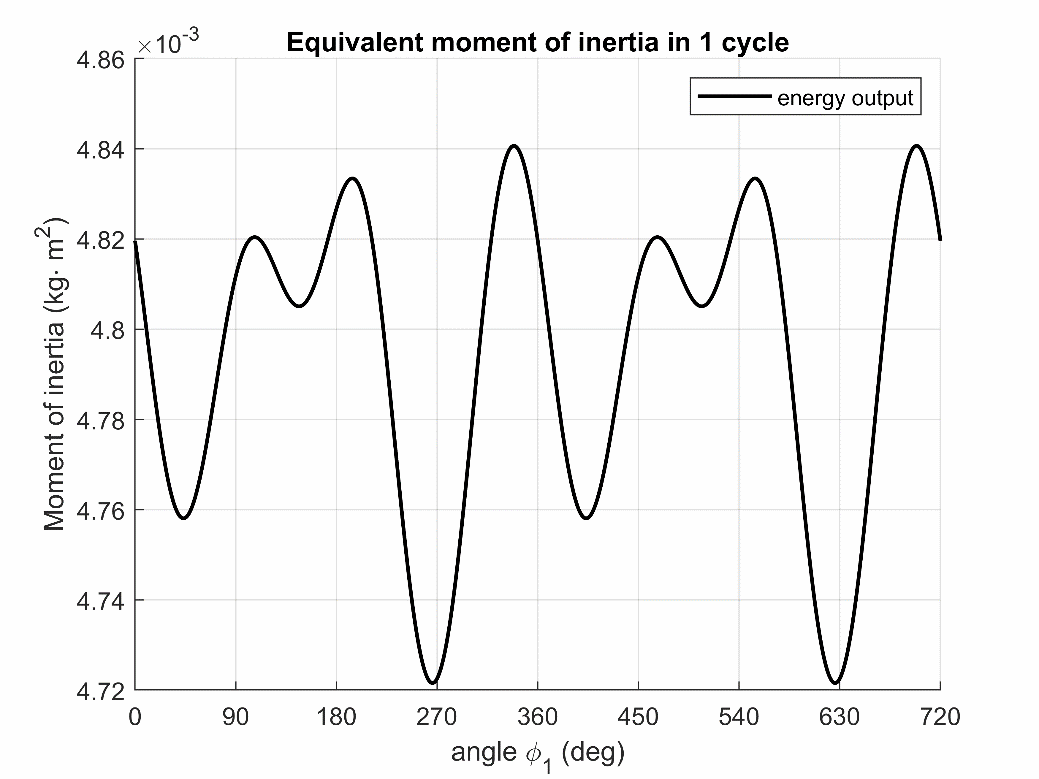
\includegraphics[width=0.6\linewidth]{19}
	\caption{Equivalent moment of inertia of the system}
	\label{fig:19}
\end{figure}\\
Then, we calculate the total energy output of the system:
\begin{equation}
	E(\phi)=\Delta E + E_0 = (A_c+A_d) + \dfrac{1}{2}J_0\omega_1^2
\end{equation}
where $ \Delta E $ is the total equivalent work and $ J_0 = J(0)$
\begin{figure}
	\centering
	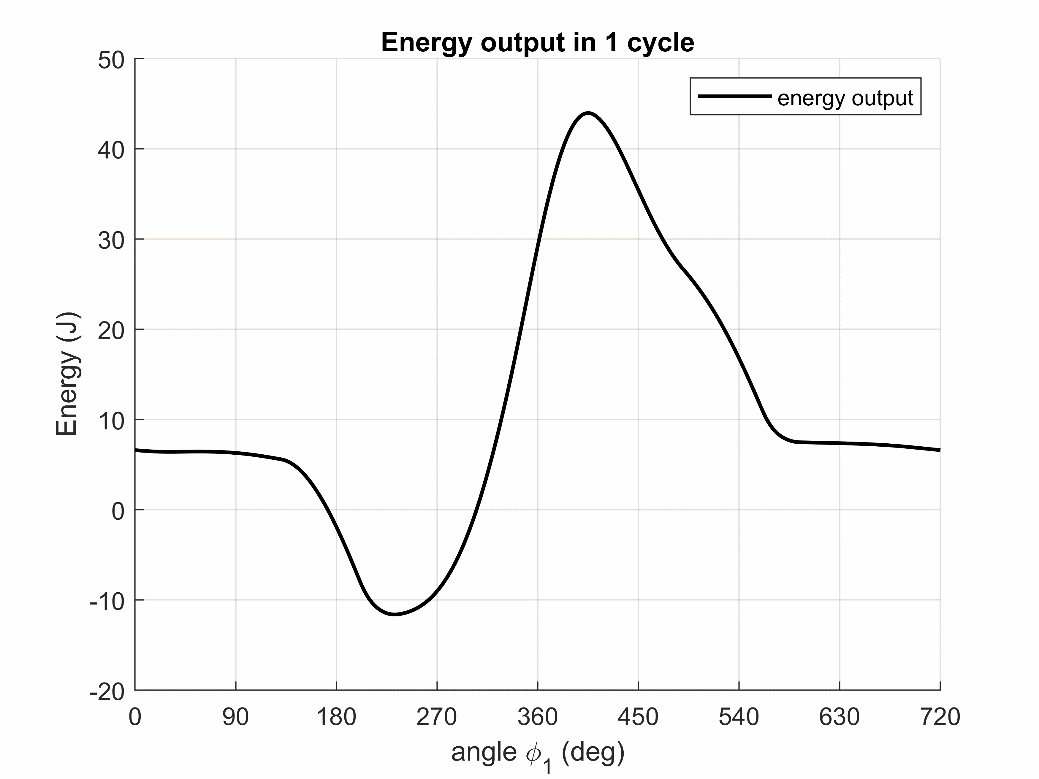
\includegraphics[width=0.6\linewidth]{20}
	\caption{Energy output of the system in 1 cycle}
	\label{fig:20}
\end{figure}\\
From the equivalent energy equation $ E(\phi) $ and moment of inertia $ J(\phi) $ we plot the graph of $ E(J) $
\begin{figure}[h]
	\centering
	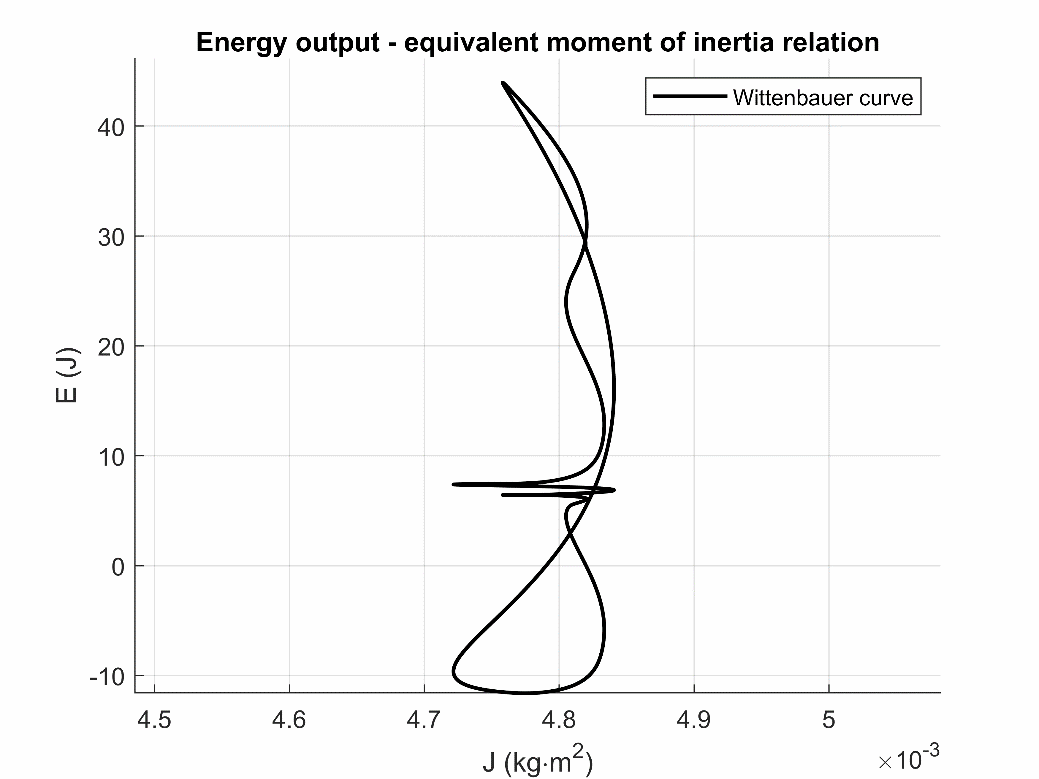
\includegraphics[width=0.6\linewidth]{21}
	\caption{Equivalent moment of inertia - energy output relations}
	\label{fig:21}
\end{figure}\\
From figure \ref{fig:21} we draw 2 tangent lines at the boundaries. Let the slope of the lower tangent line be $ \psi_{min} $ and the upper one be $ \psi_{max} $. The slope of the lines at calculated numerically as follows:
\begin{equation}
\begin{array}{c}
\psi_{min}=\dfrac{\mu_E\omega_1^2}{2\mu_J}\left(1-\dfrac{[\delta]}{2}\right)^2\\
\psi_{max}=\dfrac{\mu_E\omega_1^2}{2\mu_J}\left(1+\dfrac{[\delta]}{2}\right)^2
\end{array}
\end{equation}
\begin{tabular}{p{2cm}p{13.5cm}}
	where & $ [\delta]=1/80 $ is given above\\
	 & $ \mu_E=\mu_J =1$ are the scale of the figure (MATLAB\textup{\textregistered} or similar programs always understands these values as 1)
\end{tabular}

The lines cross the ordinate $ E(J) $ at $ a, b $ respectively. We then derive the equations describing these lines and draw them in figure \ref{fig:21}:
\begin{equation}
	\begin{array}{c}
	y_{min}=\psi_{min} x + a\\
	y_{max}=\psi_{max} x + b
	\end{array}
\end{equation}
\begin{figure}
	\centering
	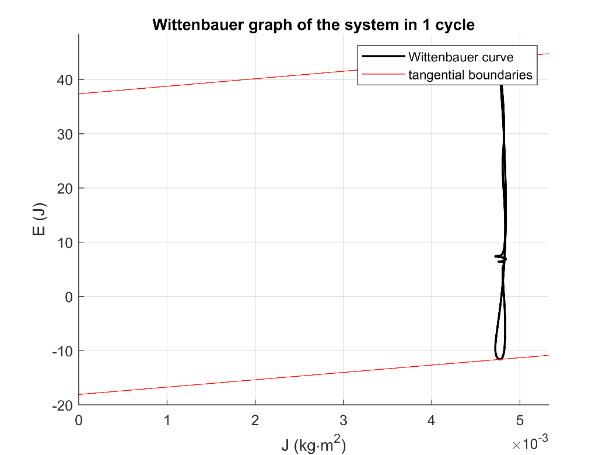
\includegraphics[width=0.6\linewidth]{22}
	\caption{Wittenbauer curve with tangent boundaries}
	\label{fig:22}
\end{figure}
Calculating the moment of inertia of the flywheel using:
\begin{equation}
	J_d=\dfrac{\mu_J ab}{\psi_{max}-\psi_{min}}
\end{equation}
Programming with MATLAB\textup{\textregistered}, we estimate $ J_d=1.63\unit{kg\cdot m^2} $. Assuming the cross section area is $ 100\unit{cm^2} $, the weight of the flywheel will be about $ 16.3\unit{g} $.
\section{Combining motion of the system}
From the given parameters, we derive the following table:
\begin{figure}[h]
	\centering
	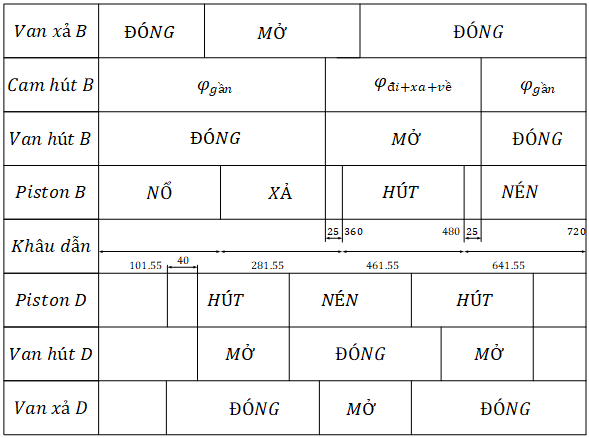
\includegraphics[width=0.6\linewidth]{23}
	\caption{Timing chart of the system}
	\label{fig:23}
\end{figure}
\section{Cam mechanism}
\subsection{Tasks}
\begin{itemize}
	\item Modeling 4 cams for 4 valves, 2 of which are intake-outtake of the combustion end, and the remaining are for the compression end.
	\item The intake cams are identical.
	\item The outtake cams are identical.
\end{itemize}
\subsection{Cam profile determination}
For combustion ends, we will find the rise, dwell, fall of the motion:
\[\phi_{rise,comb}+\phi_{dwell,comb}+\phi_{fall,comb}=\dfrac{230^\circ}{2}=115^\circ\]
\[\Rightarrow\left\{\begin{array}{ll}
\phi_{rise,comb}&=55^\circ\\
\phi_{dwell,comb}&=5^\circ\\
\phi_{fall,comb}&=55^\circ\\
\end{array}\right.\]
Knowing the angles of each interval and the form of acceleration (modified trapezoidal), we can integrate to find velocity and displacement of the cam follower. For vibration safety, jerk is included using derivative with respect to $ \phi(t) $
\begin{figure}[h]
	\centering
	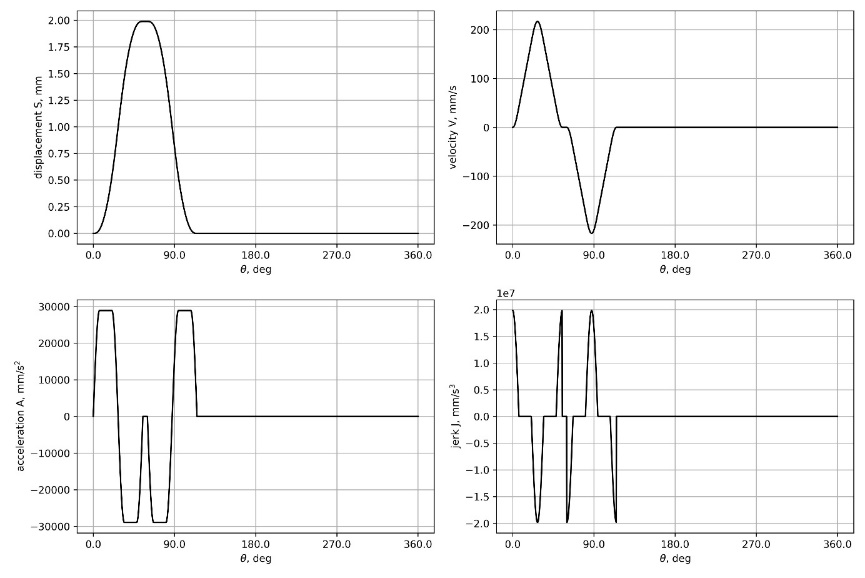
\includegraphics[width=0.8\linewidth]{24}
	\caption{Displacement, velocity, acceleration and jerk of the cam follower}
	\label{fig:24}
\end{figure}\\
For flat faced follower, the pressure angle is constant. This leads to the condition of convex cam profile $ R_0+Y+\frac{dY^2}{d\phi}>0 $ or:
\begin{equation}\label{camc}
	R_0> h_{max}
\end{equation}
where $ h_{max} $ is the minimum value of the sum $ Y+\frac{dY^2}{d\phi} $.\\
From the figure, $ h_{max}=9.096\unit{mm} $. Then, arbitrarily choose $ R_0=12\unit{mm} $ to satisfy the condition (\ref{camc}).
% TODO: \usepackage{graphicx} required
\begin{figure}[h]
	\centering
	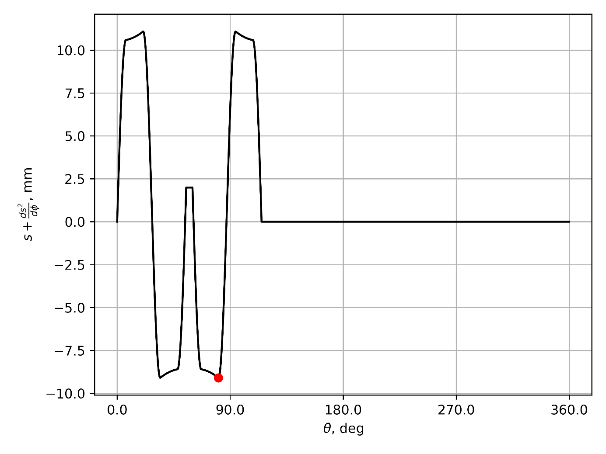
\includegraphics[width=0.6\linewidth]{25}
	\caption{Displacement - acceleration diagram of the cam}
	\label{fig:25}
\end{figure}\\
From the pressure angle $ \alpha_2=6^\circ $, we use superposition to create an equivalent cam profile, namely $ Y=Y\cos\alpha_2 $. Then, apply the following formula to find cam profile:
\begin{equation}
\left\{
\begin{array}{ll}
u&=(R_0+Y)\sin\phi + Y'\cos\phi\\
v&=(R_0+Y)\cos\phi - Y'\sin\phi
\end{array}
\right.
\end{equation}
where $ \phi(t) =\widehat{xOA}$; $ u,v $ are the position of cam along $ x,y $-axes respectively; $ Y,Y' $ are the displacement and velocity of the cam follower as shown in figure \ref{fig:24}.
\begin{figure}[h]
	\centering
	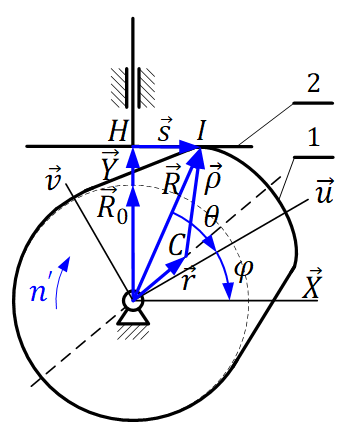
\includegraphics[width=0.4\linewidth]{26}
	\caption{Position vectors of the cam}
	\label{fig:26}
\end{figure}\\
Using MATLAB\textup{\textregistered}, we plot the cam profile numerically. Applying this process to the compression end, we also plot the cam profile in figure \ref{fig:28}:
\begin{figure}[h]
	\centering
	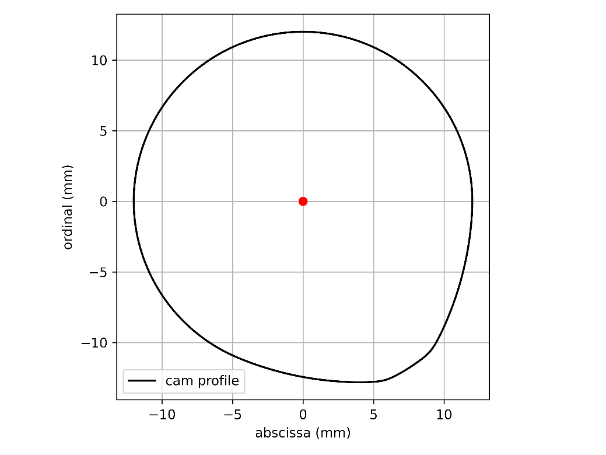
\includegraphics[width=0.6\linewidth]{27}
	\caption{Cam profile of the combustion end}
	\label{fig:27}
\end{figure}
\begin{figure}[h]
	\centering
	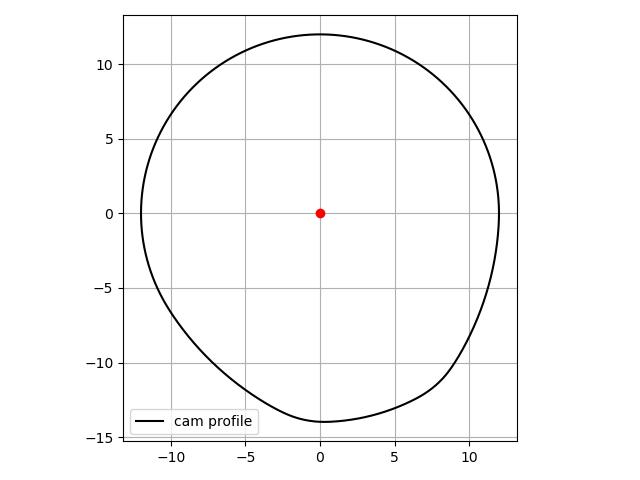
\includegraphics[width=0.6\linewidth]{28}
	\caption{Cam profile of the compression end}
	\label{fig:28}
\end{figure}